% P05 training-only smoke figure; not a model comparison on unseen data.
% data_sha256=48e1a384f932994448b539ec2f8e8de886893170c1f8f952359914470f815f3f
\documentclass[tikz,border=8pt]{standalone}
\usepackage{pgfplots}
\pgfplotsset{compat=1.18}
\usepgfplotslibrary{groupplots}
\ifdefined\pdfinfoomitdate\pdfinfoomitdate=1\fi
\ifdefined\pdfsuppressptexinfo\pdfsuppressptexinfo=-1\fi
\ifdefined\pdftrailerid\pdftrailerid{}\fi
\definecolor{p05Dzero}{HTML}{0072B2}
\definecolor{p05Done}{HTML}{E69F00}
\definecolor{p05Dtwo}{HTML}{009E73}
\definecolor{p05Dthree}{HTML}{CC79A7}
\begin{document}
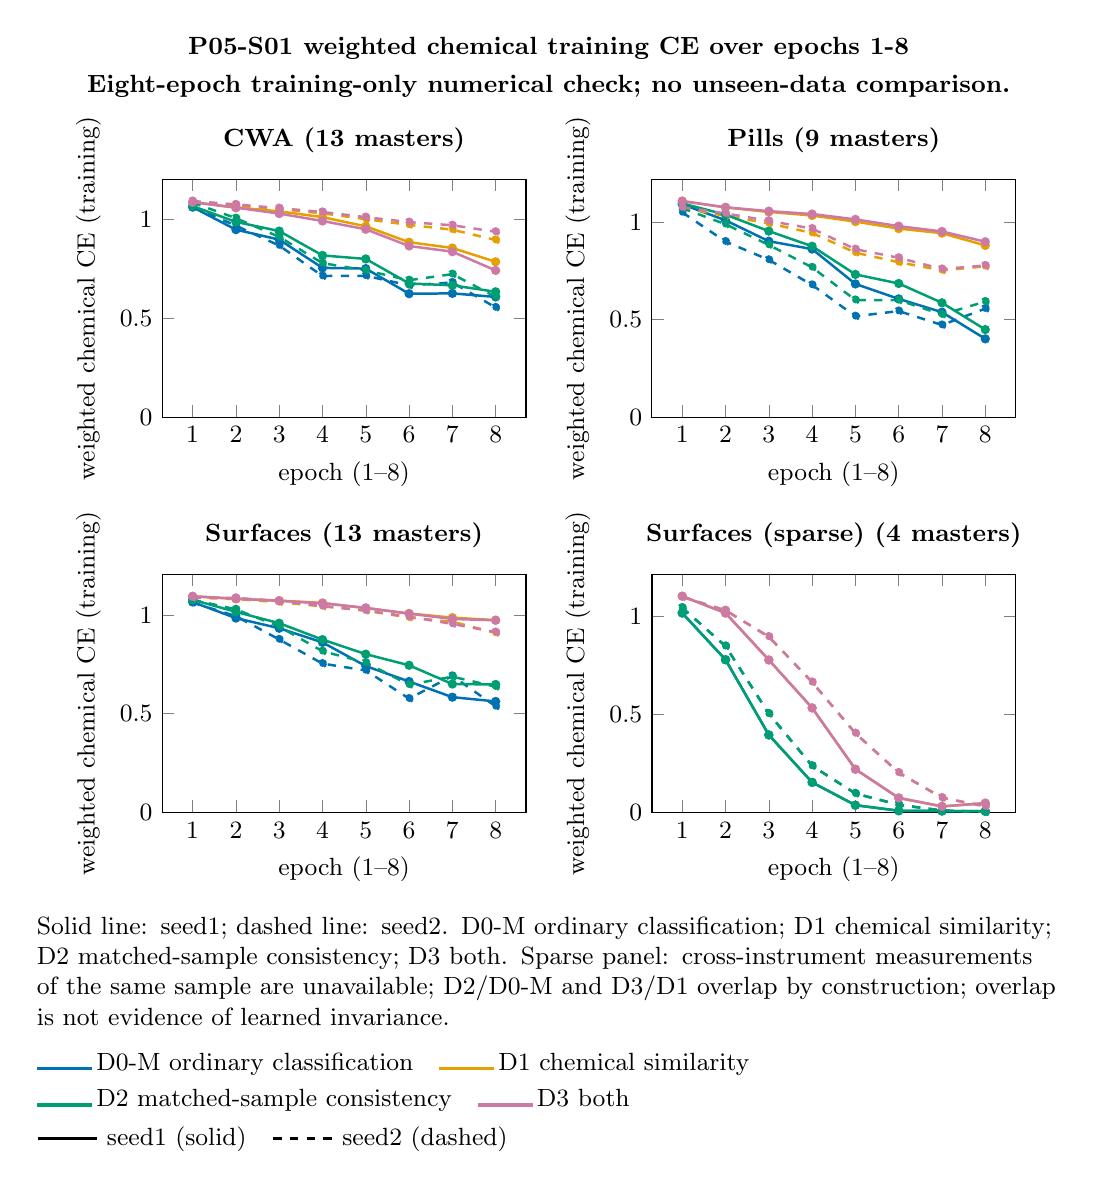
\begin{tikzpicture}
\begin{groupplot}[
  group style={group size=2 by 2, xlabels at=edge bottom, ylabels at=edge left, horizontal sep=1.6cm, vertical sep=2.0cm},
  width=6.2cm, height=4.6cm,
  every axis plot/.append style={line width=0.9pt},
  tick label style={font=\small, color=black},
  label style={font=\small, color=black},
  title style={font=\small\bfseries, color=black},
]
\nextgroupplot[title={CWA (13 masters)}, xlabel={epoch (1--8)}, ylabel={weighted chemical CE (training)}, xtick={1,...,8}, ymin=0]
\addplot[color=p05Dzero, solid, mark=*, mark size=1.2pt] coordinates {(1,1.0626162886619568) (2,0.9486355185508728) (3,0.89812348783016205) (4,0.75515483319759369) (5,0.75148618221282959) (6,0.62436778843402863) (7,0.62602980434894562) (8,0.60807578265666962)};
\addplot[color=p05Dzero, dashed, mark=*, mark size=1.2pt] coordinates {(1,1.0634686350822449) (2,0.96862533688545227) (3,0.86824913322925568) (4,0.71388678252696991) (5,0.71519090235233307) (6,0.66669391095638275) (7,0.68135988712310791) (8,0.5547143742442131)};
\addplot[color=p05Done, solid, mark=*, mark size=1.2pt] coordinates {(1,1.0883093476295471) (2,1.0605588257312775) (3,1.0413568317890167) (4,1.0118670016527176) (5,0.96540530025959015) (6,0.88520193099975586) (7,0.855818971991539) (8,0.78602668642997742)};
\addplot[color=p05Done, dashed, mark=*, mark size=1.2pt] coordinates {(1,1.090491771697998) (2,1.0676590800285339) (3,1.0533806979656219) (4,1.0313538908958435) (5,1.001811146736145) (6,0.97277453541755676) (7,0.94864962995052338) (8,0.89596922695636749)};
\addplot[color=p05Dtwo, solid, mark=*, mark size=1.2pt] coordinates {(1,1.0677400231361389) (2,0.98788614571094513) (3,0.94157569110393524) (4,0.81815697252750397) (5,0.80049914121627808) (6,0.67635433375835419) (7,0.66688133776187897) (8,0.63416217267513275)};
\addplot[color=p05Dtwo, dashed, mark=*, mark size=1.2pt] coordinates {(1,1.0856600403785706) (2,1.0066143870353699) (3,0.91198602318763733) (4,0.77935592830181122) (5,0.74237628281116486) (6,0.69279022514820099) (7,0.72342613339424133) (8,0.60857880115509033)};
\addplot[color=p05Dthree, solid, mark=*, mark size=1.2pt] coordinates {(1,1.0872949063777924) (2,1.0598500669002533) (3,1.0299900770187378) (4,0.99244271218776703) (5,0.95042197406291962) (6,0.86591903865337372) (7,0.83717916905879974) (8,0.74223130941390991)};
\addplot[color=p05Dthree, dashed, mark=*, mark size=1.2pt] coordinates {(1,1.0935605764389038) (2,1.0763550996780396) (3,1.057628333568573) (4,1.0380687713623047) (5,1.0119019895792007) (6,0.98666572570800781) (7,0.97090065479278564) (8,0.93772518634796143)};
\nextgroupplot[title={Pills (9 masters)}, xlabel={epoch (1--8)}, ylabel={weighted chemical CE (training)}, xtick={1,...,8}, ymin=0]
\addplot[color=p05Dzero, solid, mark=*, mark size=1.2pt] coordinates {(1,1.0929531157016754) (2,1.0104851126670837) (3,0.90316365659236908) (4,0.86265678703784943) (5,0.68373757600784302) (6,0.60700562596321106) (7,0.53865624219179153) (8,0.40175881236791611)};
\addplot[color=p05Dzero, dashed, mark=*, mark size=1.2pt] coordinates {(1,1.0513689517974854) (2,0.90115702152252197) (3,0.80743344128131866) (4,0.67856623232364655) (5,0.51775680482387543) (6,0.54443596303462982) (7,0.47288027405738831) (8,0.55703215301036835)};
\addplot[color=p05Done, solid, mark=*, mark size=1.2pt] coordinates {(1,1.109565794467926) (2,1.0766449570655823) (3,1.05343297123909) (4,1.0352360308170319) (5,1.0038649588823318) (6,0.96795611083507538) (7,0.94443085789680481) (8,0.88160768151283264)};
\addplot[color=p05Done, dashed, mark=*, mark size=1.2pt] coordinates {(1,1.0746818780899048) (2,1.0334807336330414) (3,0.99486580491065979) (4,0.94542530179023743) (5,0.84435030817985535) (6,0.79524436593055725) (7,0.75349721312522888) (8,0.77403049170970917)};
\addplot[color=p05Dtwo, solid, mark=*, mark size=1.2pt] coordinates {(1,1.0973517298698425) (2,1.0395639836788177) (3,0.95491884648799896) (4,0.87732866406440735) (5,0.73265464603900909) (6,0.6861000657081604) (7,0.58681681007146835) (8,0.44939827919006348)};
\addplot[color=p05Dtwo, dashed, mark=*, mark size=1.2pt] coordinates {(1,1.072840541601181) (2,0.9902157336473465) (3,0.88406705856323242) (4,0.76876324415206909) (5,0.60117942094802856) (6,0.60030508041381836) (7,0.52662693709135056) (8,0.59310176968574524)};
\addplot[color=p05Dthree, solid, mark=*, mark size=1.2pt] coordinates {(1,1.1090696752071381) (2,1.0772877633571625) (3,1.0577448308467865) (4,1.0428083539009094) (5,1.0153451561927795) (6,0.98060733079910278) (7,0.95328676700592041) (8,0.90029530227184296)};
\addplot[color=p05Dthree, dashed, mark=*, mark size=1.2pt] coordinates {(1,1.0776720941066742) (2,1.0457427799701691) (3,1.0078724026679993) (4,0.96801355481147766) (5,0.86217358708381653) (6,0.81801480054855347) (7,0.76045131683349609) (8,0.77843120694160461)};
\nextgroupplot[title={Surfaces (13 masters)}, xlabel={epoch (1--8)}, ylabel={weighted chemical CE (training)}, xtick={1,...,8}, ymin=0]
\addplot[color=p05Dzero, solid, mark=*, mark size=1.2pt] coordinates {(1,1.0663981437683105) (2,0.98475760221481323) (3,0.93335223197937012) (4,0.86147111654281616) (5,0.74146692454814911) (6,0.66314829885959625) (7,0.5836806446313858) (8,0.56215117871761322)};
\addplot[color=p05Dzero, dashed, mark=*, mark size=1.2pt] coordinates {(1,1.0632773637771606) (2,0.99466085433959961) (3,0.87637743353843689) (4,0.75389967858791351) (5,0.71926748752593994) (6,0.57635657489299774) (7,0.69145017862319946) (8,0.53726047277450562)};
\addplot[color=p05Done, solid, mark=*, mark size=1.2pt] coordinates {(1,1.0945394337177277) (2,1.0825395286083221) (3,1.0735869109630585) (4,1.0617660880088806) (5,1.0350788831710815) (6,1.0081778764724731) (7,0.9870888888835907) (8,0.97430111467838287)};
\addplot[color=p05Done, dashed, mark=*, mark size=1.2pt] coordinates {(1,1.0883212089538574) (2,1.0814889967441559) (3,1.0656233429908752) (4,1.0444225966930389) (5,1.0230598449707031) (6,0.98739846050739288) (7,0.96603609621524811) (8,0.90993195772171021)};
\addplot[color=p05Dtwo, solid, mark=*, mark size=1.2pt] coordinates {(1,1.0780039727687836) (2,1.01629339158535) (3,0.95899015665054321) (4,0.87571661174297333) (5,0.80178757011890411) (6,0.7454599142074585) (7,0.65028771758079529) (8,0.64816772937774658)};
\addplot[color=p05Dtwo, dashed, mark=*, mark size=1.2pt] coordinates {(1,1.0777319371700287) (2,1.0292570441961288) (3,0.94194655120372772) (4,0.81673991680145264) (5,0.75923062860965729) (6,0.64688518643379211) (7,0.68765874207019806) (8,0.63698971271514893)};
\addplot[color=p05Dthree, solid, mark=*, mark size=1.2pt] coordinates {(1,1.0960149466991425) (2,1.0831278860569) (3,1.0723001658916473) (4,1.0597701370716095) (5,1.0369396805763245) (6,1.0072827339172363) (7,0.98035342991352081) (8,0.97378070652484894)};
\addplot[color=p05Dthree, dashed, mark=*, mark size=1.2pt] coordinates {(1,1.0889257192611694) (2,1.0874022543430328) (3,1.0711941123008728) (4,1.0463317930698395) (5,1.0230007618665695) (6,0.99207864701747894) (7,0.95520250499248505) (8,0.91371116042137146)};
\nextgroupplot[title={Surfaces (sparse) (4 masters)}, xlabel={epoch (1--8)}, ylabel={weighted chemical CE (training)}, xtick={1,...,8}, ymin=0]
\addplot[color=p05Dzero, solid, mark=*, mark size=1.2pt] coordinates {(1,1.0180680751800537) (2,0.77921652793884277) (3,0.39497798681259155) (4,0.15259058959782124) (5,0.036011567804962397) (6,0.0076324696419760585) (7,0.0062511647120118141) (8,0.0050914695020765066)};
\addplot[color=p05Dzero, dashed, mark=*, mark size=1.2pt] coordinates {(1,1.0447807312011719) (2,0.84899435937404633) (3,0.50376061350107193) (4,0.23698116466403008) (5,0.095700918696820736) (6,0.037955246749334037) (7,0.0089130678679794073) (8,0.0013501324428943917)};
\addplot[color=p05Done, solid, mark=*, mark size=1.2pt] coordinates {(1,1.1041192710399628) (2,1.01786869764328) (3,0.77823561429977417) (4,0.53316929936408997) (5,0.21978765726089478) (6,0.073133429512381554) (7,0.02976234583184123) (8,0.04634437058120966)};
\addplot[color=p05Done, dashed, mark=*, mark size=1.2pt] coordinates {(1,1.1003016233444214) (2,1.0317001193761826) (3,0.89680947363376617) (4,0.66488628089427948) (5,0.40352458879351616) (6,0.20228475332260132) (7,0.074103505350649357) (8,0.030303581617772579)};
\addplot[color=p05Dtwo, solid, mark=*, mark size=1.2pt] coordinates {(1,1.0180680751800537) (2,0.77921652793884277) (3,0.39497798681259155) (4,0.15259058959782124) (5,0.036011567804962397) (6,0.0076324696419760585) (7,0.0062511647120118141) (8,0.0050914695020765066)};
\addplot[color=p05Dtwo, dashed, mark=*, mark size=1.2pt] coordinates {(1,1.0447807312011719) (2,0.84899435937404633) (3,0.50376061350107193) (4,0.23698116466403008) (5,0.095700918696820736) (6,0.037955246749334037) (7,0.0089130678679794073) (8,0.0013501324428943917)};
\addplot[color=p05Dthree, solid, mark=*, mark size=1.2pt] coordinates {(1,1.1041192710399628) (2,1.01786869764328) (3,0.77823561429977417) (4,0.53316929936408997) (5,0.21978765726089478) (6,0.073133429512381554) (7,0.02976234583184123) (8,0.04634437058120966)};
\addplot[color=p05Dthree, dashed, mark=*, mark size=1.2pt] coordinates {(1,1.1003016233444214) (2,1.0317001193761826) (3,0.89680947363376617) (4,0.66488628089427948) (5,0.40352458879351616) (6,0.20228475332260132) (7,0.074103505350649357) (8,0.030303581617772579)};
\end{groupplot}
\node[anchor=south, font=\bfseries\small, color=black, align=center, text width=13cm] at (current bounding box.north) {P05-S01 weighted chemical training CE over epochs 1-8\\[1mm]Eight-epoch training-only numerical check; no unseen-data comparison.};
\node[anchor=north, font=\small, color=black, align=left, text width=13cm] (p05caption) at ([yshift=-2mm]current bounding box.south) {Solid line: seed1; dashed line: seed2. D0-M ordinary classification; D1 chemical similarity; D2 matched-sample consistency; D3 both. Sparse panel: cross-instrument measurements of the same sample are unavailable; D2/D0-M and D3/D1 overlap by construction; overlap is not evidence of learned invariance.};
\node[anchor=north west, font=\small, color=black, align=left, text width=13cm] at ([yshift=-1mm]p05caption.south west) {\textcolor{p05Dzero}{\rule{7mm}{1.2pt}}\,D0-M ordinary classification\quad \textcolor{p05Done}{\rule{7mm}{1.2pt}}\,D1 chemical similarity\\[0.8mm]\textcolor{p05Dtwo}{\rule{7mm}{1.2pt}}\,D2 matched-sample consistency\quad \textcolor{p05Dthree}{\rule{7mm}{1.2pt}}\,D3 both\\[1mm]\tikz[baseline=-0.6ex]\draw[black,solid,line width=0.9pt](0,0)--(0.75,0);\ seed1 (solid)\quad \tikz[baseline=-0.6ex]\draw[black,dashed,line width=0.9pt](0,0)--(0.75,0);\ seed2 (dashed)};
\end{tikzpicture}
\end{document}
